\documentclass[twoside]{book}

% Packages required by doxygen
\usepackage{calc}
\usepackage{doxygen}
\usepackage{graphicx}
\usepackage[utf8]{inputenc}
\usepackage{makeidx}
\usepackage{multicol}
\usepackage{multirow}
\usepackage{textcomp}
\usepackage[table]{xcolor}

% Font selection
\usepackage[T1]{fontenc}
\usepackage{mathptmx}
\usepackage[scaled=.90]{helvet}
\usepackage{courier}
\usepackage{amssymb}
\usepackage{sectsty}
\renewcommand{\familydefault}{\sfdefault}
\allsectionsfont{%
  \fontseries{bc}\selectfont%
  \color{darkgray}%
}
\renewcommand{\DoxyLabelFont}{%
  \fontseries{bc}\selectfont%
  \color{darkgray}%
}

% Page & text layout
\usepackage{geometry}
\geometry{%
  a4paper,%
  top=2.5cm,%
  bottom=2.5cm,%
  left=2.5cm,%
  right=2.5cm%
}
\tolerance=750
\hfuzz=15pt
\hbadness=750
\setlength{\emergencystretch}{15pt}
\setlength{\parindent}{0cm}
\setlength{\parskip}{0.2cm}
\makeatletter
\renewcommand{\paragraph}{%
  \@startsection{paragraph}{4}{0ex}{-1.0ex}{1.0ex}{%
    \normalfont\normalsize\bfseries\SS@parafont%
  }%
}
\renewcommand{\subparagraph}{%
  \@startsection{subparagraph}{5}{0ex}{-1.0ex}{1.0ex}{%
    \normalfont\normalsize\bfseries\SS@subparafont%
  }%
}
\makeatother

% Headers & footers
\usepackage{fancyhdr}
\pagestyle{fancyplain}
\fancyhead[LE]{\fancyplain{}{\bfseries\thepage}}
\fancyhead[CE]{\fancyplain{}{}}
\fancyhead[RE]{\fancyplain{}{\bfseries\leftmark}}
\fancyhead[LO]{\fancyplain{}{\bfseries\rightmark}}
\fancyhead[CO]{\fancyplain{}{}}
\fancyhead[RO]{\fancyplain{}{\bfseries\thepage}}
\fancyfoot[LE]{\fancyplain{}{}}
\fancyfoot[CE]{\fancyplain{}{}}
\fancyfoot[RE]{\fancyplain{}{\bfseries\scriptsize Generated on Fri Dec 6 2013 20\-:48\-:01 for U\-I\-C Desktop App by Doxygen }}
\fancyfoot[LO]{\fancyplain{}{\bfseries\scriptsize Generated on Fri Dec 6 2013 20\-:48\-:01 for U\-I\-C Desktop App by Doxygen }}
\fancyfoot[CO]{\fancyplain{}{}}
\fancyfoot[RO]{\fancyplain{}{}}
\renewcommand{\footrulewidth}{0.4pt}
\renewcommand{\chaptermark}[1]{%
  \markboth{#1}{}%
}
\renewcommand{\sectionmark}[1]{%
  \markright{\thesection\ #1}%
}

% Indices & bibliography
\usepackage{natbib}
\usepackage[titles]{tocloft}
\setcounter{tocdepth}{3}
\setcounter{secnumdepth}{5}
\makeindex

% Hyperlinks (required, but should be loaded last)
\usepackage{ifpdf}
\ifpdf
  \usepackage[pdftex,pagebackref=true]{hyperref}
\else
  \usepackage[ps2pdf,pagebackref=true]{hyperref}
\fi
\hypersetup{%
  colorlinks=true,%
  linkcolor=blue,%
  citecolor=blue,%
  unicode%
}

% Custom commands
\newcommand{\clearemptydoublepage}{%
  \newpage{\pagestyle{empty}\cleardoublepage}%
}


%===== C O N T E N T S =====

\begin{document}

% Titlepage & ToC
\hypersetup{pageanchor=false}
\pagenumbering{roman}
\begin{titlepage}
\vspace*{7cm}
\begin{center}%
{\Large U\-I\-C Desktop App }\\
\vspace*{1cm}
{\large Generated by Doxygen 1.8.5}\\
\vspace*{0.5cm}
{\small Fri Dec 6 2013 20:48:01}\\
\end{center}
\end{titlepage}
\clearemptydoublepage
\tableofcontents
\clearemptydoublepage
\pagenumbering{arabic}
\hypersetup{pageanchor=true}

%--- Begin generated contents ---
\chapter{Hierarchical Index}
\section{Class Hierarchy}
This inheritance list is sorted roughly, but not completely, alphabetically\-:\begin{DoxyCompactList}
\item \contentsline{section}{location\-Loader}{\pageref{classlocation_loader}}{}
\item Q\-Frame\begin{DoxyCompactList}
\item \contentsline{section}{My\-Frame}{\pageref{class_my_frame}}{}
\end{DoxyCompactList}
\item Q\-Main\-Window\begin{DoxyCompactList}
\item \contentsline{section}{Main\-Window}{\pageref{class_main_window}}{}
\end{DoxyCompactList}
\item Q\-Push\-Button\begin{DoxyCompactList}
\item \contentsline{section}{My\-Push\-Button}{\pageref{class_my_push_button}}{}
\end{DoxyCompactList}
\end{DoxyCompactList}

\chapter{Class Index}
\section{Class List}
Here are the classes, structs, unions and interfaces with brief descriptions\-:\begin{DoxyCompactList}
\item\contentsline{section}{\hyperlink{classhtml_parser}{html\-Parser} }{\pageref{classhtml_parser}}{}
\item\contentsline{section}{\hyperlink{classlocation_loader}{location\-Loader} }{\pageref{classlocation_loader}}{}
\item\contentsline{section}{\hyperlink{classmenu_loader}{menu\-Loader} }{\pageref{classmenu_loader}}{}
\item\contentsline{section}{\hyperlink{classmenu_parser}{menu\-Parser} }{\pageref{classmenu_parser}}{}
\end{DoxyCompactList}

\chapter{Class Documentation}
\hypertarget{classlocation_loader}{\section{location\-Loader Class Reference}
\label{classlocation_loader}\index{location\-Loader@{location\-Loader}}
}
\subsection*{Public Member Functions}
\begin{DoxyCompactItemize}
\item 
\hypertarget{classlocation_loader_a74cd7af4aead43b9f386c6380ec6d0d1}{string {\bfseries location\-Load} (char $\ast$filename, int option)}\label{classlocation_loader_a74cd7af4aead43b9f386c6380ec6d0d1}

\item 
\hypertarget{classlocation_loader_a92c33524e9b6ad3e4eba63fd4bc2ec13}{int {\bfseries extract\-O\-Time} (string input)}\label{classlocation_loader_a92c33524e9b6ad3e4eba63fd4bc2ec13}

\item 
\hypertarget{classlocation_loader_ab513c5f807626e249e9b6d8e4006c808}{int {\bfseries extract\-C\-Time} (string input)}\label{classlocation_loader_ab513c5f807626e249e9b6d8e4006c808}

\item 
\hypertarget{classlocation_loader_a022375124026162ddeb9cc6f2060f033}{string {\bfseries extract\-Name} (string input)}\label{classlocation_loader_a022375124026162ddeb9cc6f2060f033}

\item 
\hypertarget{classlocation_loader_ac04f41072f73e10521abd3b320d3b345}{int {\bfseries extract\-O\-Time} (Q\-String input)}\label{classlocation_loader_ac04f41072f73e10521abd3b320d3b345}

\item 
\hypertarget{classlocation_loader_a8067d9ac015d2973deeb0f0ba13c0c8a}{int {\bfseries extract\-C\-Time} (Q\-String input)}\label{classlocation_loader_a8067d9ac015d2973deeb0f0ba13c0c8a}

\item 
\hypertarget{classlocation_loader_ae3c8d2242868ca7dd3ee02c77f77fdbe}{Q\-String {\bfseries location\-Load} (Q\-String filename, int option)}\label{classlocation_loader_ae3c8d2242868ca7dd3ee02c77f77fdbe}

\end{DoxyCompactItemize}


The documentation for this class was generated from the following files\-:\begin{DoxyCompactItemize}
\item 
include/location\-Loader.\-h\item 
R\-E\-M\-A\-D\-E F\-O\-R Q\-T (not standalone)/locationloader.\-h\item 
R\-E\-M\-A\-D\-E F\-O\-R Q\-T (not standalone)/locationloader.\-cpp\item 
src/location\-Loader.\-cpp\end{DoxyCompactItemize}

\hypertarget{class_main_window}{\section{Main\-Window Class Reference}
\label{class_main_window}\index{Main\-Window@{Main\-Window}}
}
Inheritance diagram for Main\-Window\-:\begin{figure}[H]
\begin{center}
\leavevmode
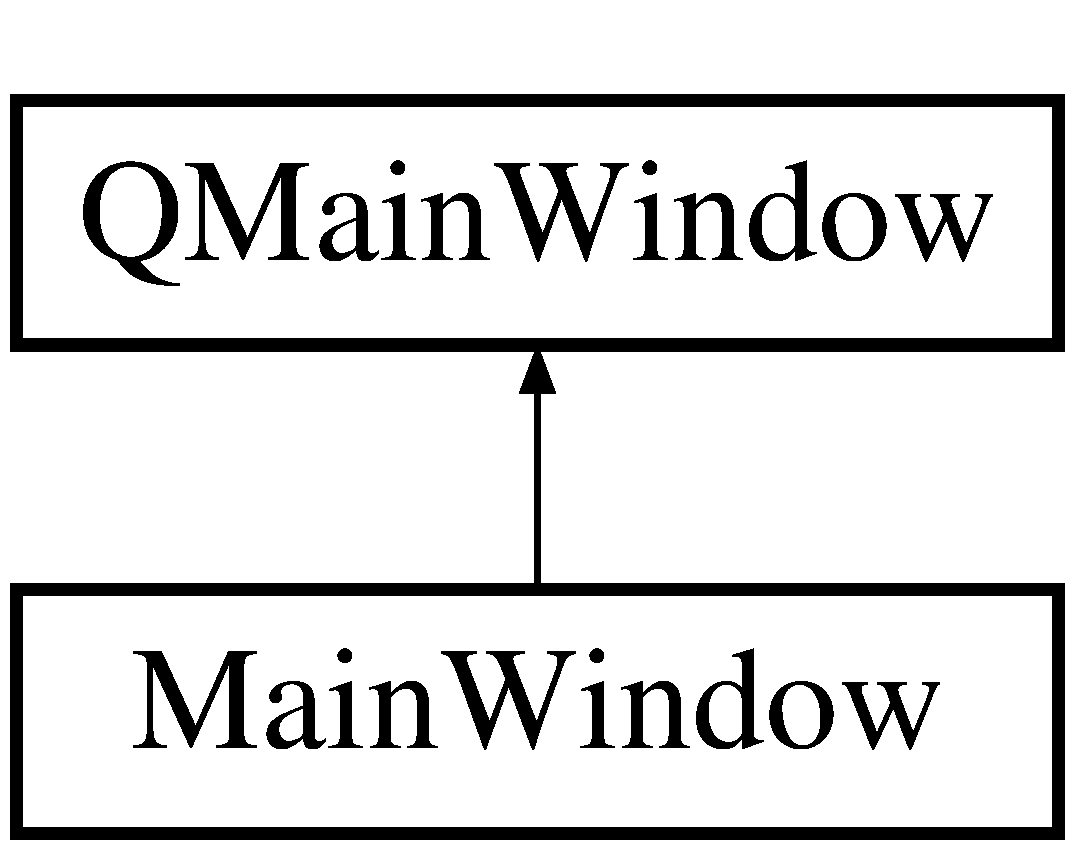
\includegraphics[height=2.000000cm]{class_main_window}
\end{center}
\end{figure}
\subsection*{Public Member Functions}
\begin{DoxyCompactItemize}
\item 
\hypertarget{class_main_window_a8b244be8b7b7db1b08de2a2acb9409db}{{\bfseries Main\-Window} (Q\-Widget $\ast$parent=0)}\label{class_main_window_a8b244be8b7b7db1b08de2a2acb9409db}

\end{DoxyCompactItemize}


The documentation for this class was generated from the following files\-:\begin{DoxyCompactItemize}
\item 
mainwindow.\-h\item 
mainwindow.\-cpp\end{DoxyCompactItemize}

\hypertarget{class_my_frame}{\section{My\-Frame Class Reference}
\label{class_my_frame}\index{My\-Frame@{My\-Frame}}
}
Inheritance diagram for My\-Frame\-:\begin{figure}[H]
\begin{center}
\leavevmode
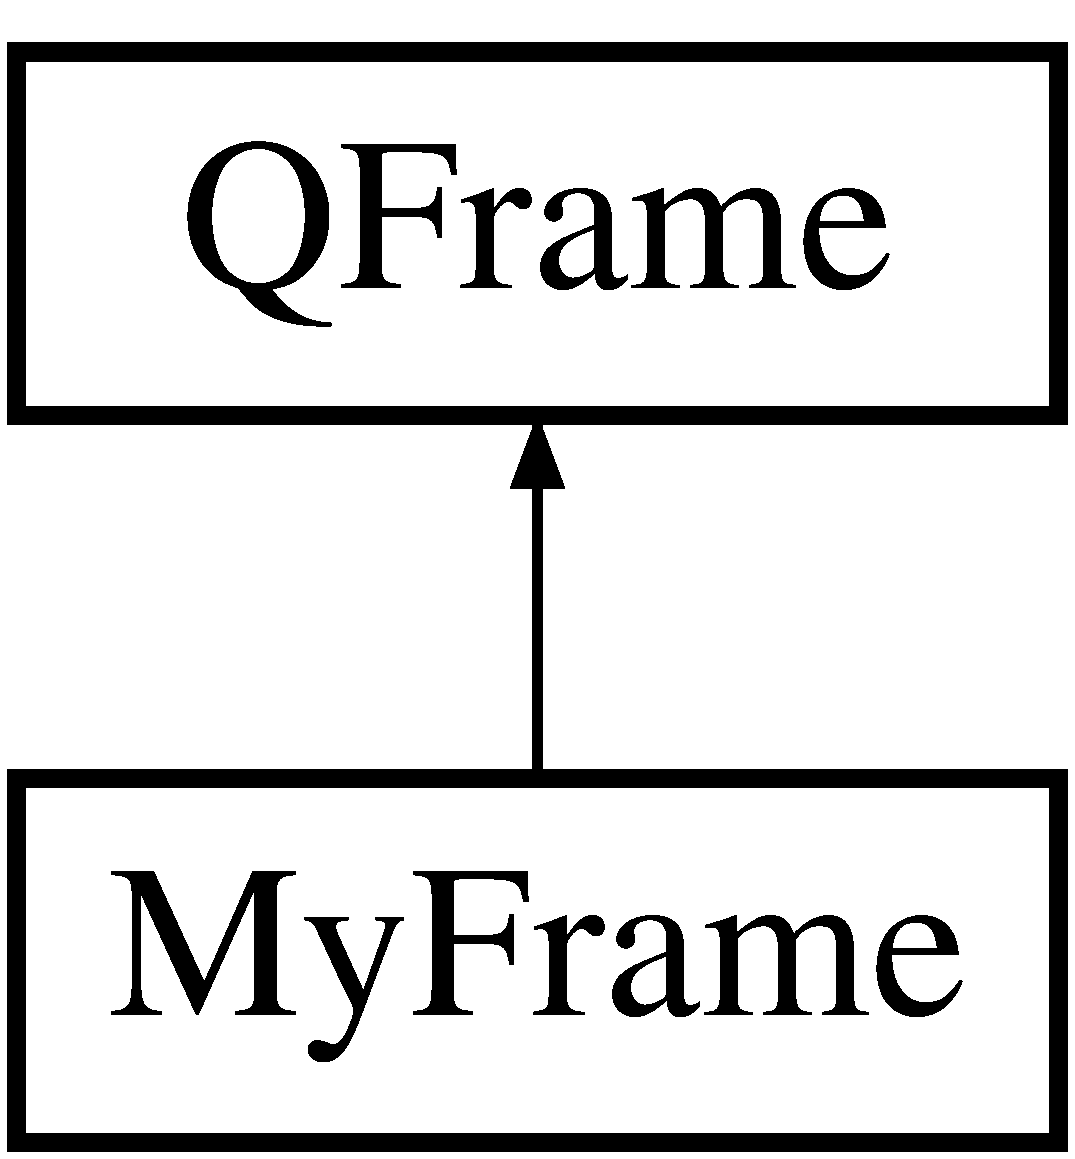
\includegraphics[height=2.000000cm]{class_my_frame}
\end{center}
\end{figure}
\subsection*{Public Member Functions}
\begin{DoxyCompactItemize}
\item 
\hypertarget{class_my_frame_ac620dfbabcc47db73f7936236e898217}{{\bfseries My\-Frame} (Q\-Widget $\ast$parent=0)}\label{class_my_frame_ac620dfbabcc47db73f7936236e898217}

\end{DoxyCompactItemize}


The documentation for this class was generated from the following files\-:\begin{DoxyCompactItemize}
\item 
myframe.\-h\item 
myframe.\-cpp\end{DoxyCompactItemize}

\hypertarget{class_my_push_button}{\section{My\-Push\-Button Class Reference}
\label{class_my_push_button}\index{My\-Push\-Button@{My\-Push\-Button}}
}
Inheritance diagram for My\-Push\-Button\-:\begin{figure}[H]
\begin{center}
\leavevmode
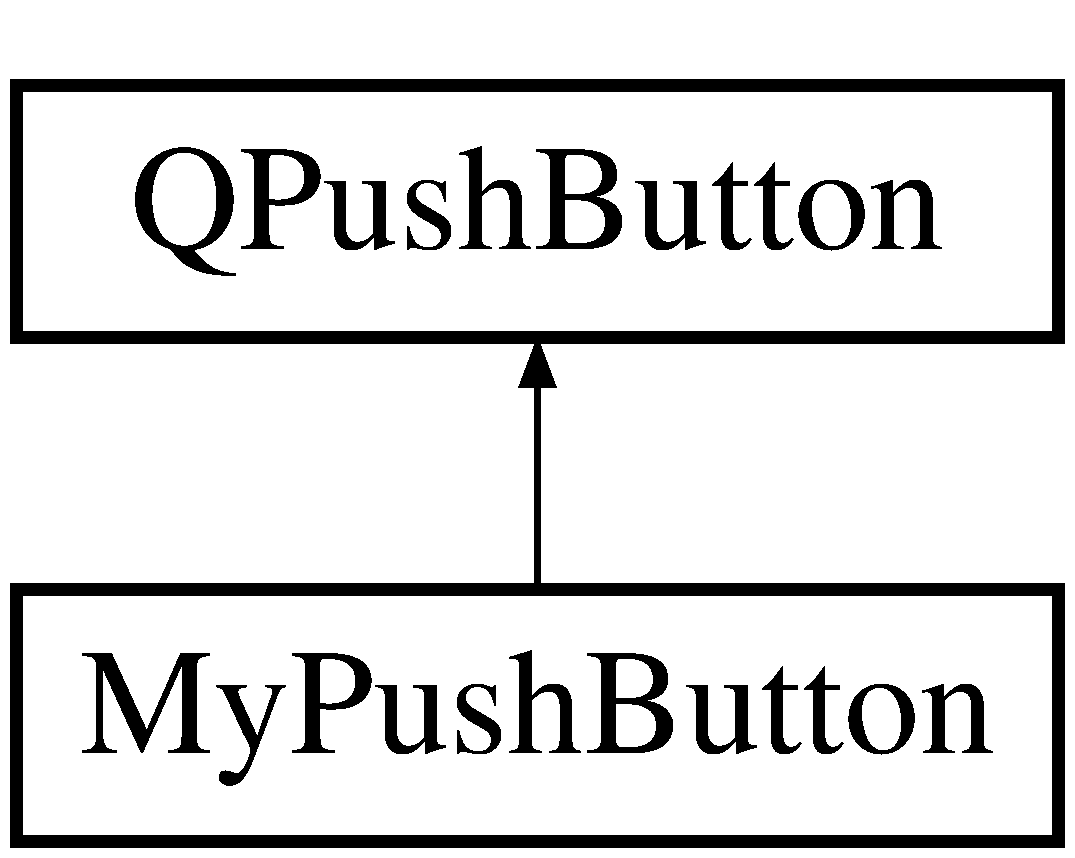
\includegraphics[height=2.000000cm]{class_my_push_button}
\end{center}
\end{figure}
\subsection*{Public Member Functions}
\begin{DoxyCompactItemize}
\item 
\hypertarget{class_my_push_button_aaebc58414627c35d593eec6912957020}{{\bfseries My\-Push\-Button} (Q\-Widget $\ast$parent=0)}\label{class_my_push_button_aaebc58414627c35d593eec6912957020}

\end{DoxyCompactItemize}


The documentation for this class was generated from the following files\-:\begin{DoxyCompactItemize}
\item 
mypushbutton.\-h\item 
mypushbutton.\-cpp\end{DoxyCompactItemize}

%--- End generated contents ---

% Index
\newpage
\phantomsection
\addcontentsline{toc}{part}{Index}
\printindex

\end{document}
